\documentclass[12pt]{article}

\usepackage{sbc-template}
\usepackage[brazil,american]{babel}
\usepackage[utf8]{inputenc}

\usepackage{graphicx}
\usepackage{url}
\usepackage{float}
\usepackage{listings}
\usepackage{color}
\usepackage{todonotes}
\usepackage{algorithmic}
\usepackage{algorithm}
\usepackage{hyperref}
\usepackage{indentfirst}
\usepackage[inline]{enumitem}

\graphicspath{{./images/}}

\sloppy

\title{Laboratório 1\\- Assembly MIPS –}

\author{Grupo 6\\
	Dayanne Fernandes da Cunha, 13/0107191\\
	Lucas Mafra Chagas, 12/0126443\\
	Marcelo Giordano Martins Costa de Oliveira, 12/0037301\\
	Lucas Junior Ribas, 16/0052289\\
	Caio Nunes de Alencar Osório, 16/0115132\\
	Diego Vaz Fernandes, 16/0117925}

\address{Dep. Ciência da Computação -- Universidade de Brasília (UnB)\\
  CiC 116394 - OAC - Turma A
  \email{}
}

\begin{document}
\maketitle

\selectlanguage{american}
 \begin{abstract}
	This report corresponds to the Experiment 1 about Assembly MIPS.
 \end{abstract}
\selectlanguage{brazil}
 \begin{resumo}
	Este relatório corresponde ao Experimento 1 sobre Assembly MIPS.
 \end{resumo}

\section{Objetivos}
\label{sec:Objetivos}

\begin{itemize}
\item Familiarizar o aluno com o Simulador/Montador MARS;
\item Desenvolver a capacidade de codificação de algoritmos em linguagem Assembly MIPS;
\item Desenvolver a capacidade de análise de desempenho de algoritmos em Assembly;
\end{itemize}

\section{Ferramentas}
\label{sec:Materiais}

\begin{itemize}
\item MARS v.4.5 Custom 7
\item Cross compiler MIPS GCC
\item Inkscape e GIMP
\end{itemize}

\section{Procedimentos}
\label{sec:Procedimentos}

Todos os códigos escritos neste laboratório podem ser encontrados no repositório \url{https://github.com/Dayof/OAC172} do \textit{GitHub}.

\subsection{Exercício 1. Simulador/Montador MARS}
\label{subsec:mars}

Esta parte do relatório foi realizada com o intuito de familiarizar os alunos ao Simulador/Montador \textit{MARS}. No item \textit{1.2} do relatório, foram pedidos os gráficos relacionados aos valores do vetor fornecido e ao tempo de execução da sub rotina \textit{Sort} fornecida pelo professor. Temos então o gráfico em melhor caso~\ref{fig:txnMC} e pior caso~\ref{fig:txnPC} da rotina de ordenação \textit{Sort}.

\begin{figure}[H]
	\centering
	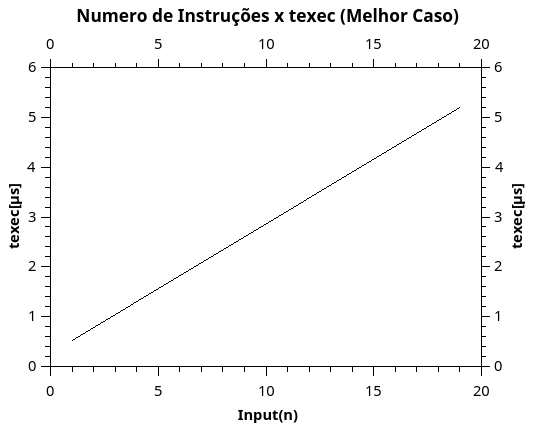
\includegraphics[width=.8\textwidth]{txnMC.png}
	\caption{n x texec(Melhor Caso)}
	\label{fig:txnMC}
\end{figure}

\begin{figure}[H]
	\centering
	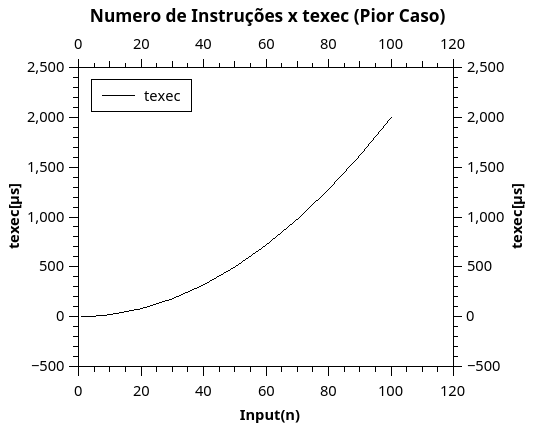
\includegraphics[width=.8\textwidth]{txnPC.png}
	\caption{n x texec(Pior Caso)}
	\label{fig:txnPC}
\end{figure}

Analisando somente os gráficos, percebemos que esse algoritmo tem tempo de execução linear em seu melhor caso, e em pior caso possui tempo de execução limitado por O(\(n^2\)), sendo representado por um braço de parábola.

\subsection{Exercício 2. Compilador GCC}
\label{subsec:comp}

Para compilar código \textit{C} em código \textit{Assembly} foi utilizado o \textit{cross compiler} \cite{MIPS} \textit{GCC}. Usando o comando \textit{\$ mips-elf-gcc -I../include -S testeX.c (X $\in$ [0,8])} foi testado a convenção para geração do código \textit{Assembly}.

\subsubsection{Diretivas}
\label{subsubsec:diretivas}

Diretivas são apenas comandos ao montador e não fazem parte do conjunto de instruções dos processadores \textit{x86}. Todas as diretivas começam com (.) (\textit{ASCII 0x2E}). Elas permitem a alocação de espaço para a declaração de variáveis " \textit{.byte}, \textit{.word} ", definição de escopo " \textit{.glob1} ", além de várias outras funções de gerenciamento como as listadas a seguir (as informações abaixo foram encontradas usando as fontes \cite{mips1}, \cite{mips2-1}, \cite{mips2-2}, \cite{mips2-3}, \cite{mips3},
\cite{mips4}, \cite{mips5} e \cite{mips6} ):

\begin{itemize}

\item .file \textit{string} : Cria uma tabela de símbolos de entrada onde a \textit{string} é o nome do símbolo e \textit{STT\_FILE} é o tipo deste símbolo, a \textit{string} especifica o nome do arquivo fonte associado ao arquivo objeto.
\item .section \textit{section}, \textit{attributes} : \textit{Section} é montado como seção atual. \textit{Attributes} é incluso se for a primeira vez que \textit{.section} é especificado.
\item .mdebug : Força a saída de depuração para entrar em uma seção .mdebug de estilo ECOFF em vez das seções padrão ELF .stabs.
\item .previous : Troca esta seção pela que foi referenciada recentemente.
\item .nan : Esta diretiva diz qual codificação \textit{MIPS} será usada para ponto flutuante IEEE 754. A primeira, padrão \textit{2008}, diz para o montador utilizar a codificação IEEE 754-2008, enquando a \textit{legacy} utiliza a codificação original do \textit{MIPS}.
\item .gnu\_attribute \textit{tag}, \textit{value} : Grava um atributo objeto \textit{gnu} para este arquivo.
\item .globl \textit{symbol1, symbol2, ..., symbolN}: Torna global cada símbolo da lista. A diretiva torna o símbolo global no escopo mas não declara o símbolo.
\item .data : Muda a seção atual para \textit{.data} (dados estáticos do programa).
\item .type \textit{symbol[, symbol, ..., symbol], type[, visibility]}: Atribui tipo ao símbolo, podendo ser do tipo função, objeto, sem tipo e um objeto \textit{TLS (Thread Local Storage)}.
\item .size \textit{symbol, expr}: Resolve expressão e atribui tamanho em bytes ao \textit{symbol}.
\item .word : Armazena o valor listado como palavras de 32 bits no limite.
\item .rdata : Adiciona dados apenas de leitura.
\item .align \textit{integer} : Ajusta o contador de locação para um valor múltiplo de 2.
\item .ascii "\textit{string}" : Aloca espaço para cadeias de caracteres sem o "\textit{$\backslash$0}".
\item .text : Muda a seção atual para \textit{.text} (instruções).
\item .ent \textit{name[,label]} : Marca o começo da função \textit{name}.
\item .frame : Descreve o quadro da pilha usada para chamar a função principal(\textit{main}).
\item .set \textit{symbol, expression}: Resolve a expressão (\textit{expression}) e atribui o valor ao símbolo (\textit{symbol}).
\item .mask \textit{mask offset} : Configura uma máscara que indica quais registradores de uso geral foram salvos na rotina atual. Esses valores são usados pelo montador para gerar a seção \textit{.reginfo} do arquivo objeto dos processadores \textit{MIPS}.
\item .fmask \textit{mask offset} : Configura uma máscara informando os registradores de ponto flutuante que a rotina atual salvou. Esses valores são usados pelo montador para gerar a seção \textit{.reginfo} do arquivo objeto dos processadores \textit{MIPS}.

\end{itemize}

\subsubsection{Assembly no MARS}
\label{subsubsec:atomars}

Algumas diretivas listadas acima não são reconhecidas pelo \textit{MARS (Mips Assembly and Runtime Simulator)}, como por exemplo \textit{.section, .previous, . nan, etc}, assim como alguns elementos como \textit{@object, @function, etc}. Logo, as seguintes instruções foram retiradas:

\begin{itemize}
\item @object\\
  \begin{itemize}
  \item .type v, @object
  \end{itemize}
 \item @function\\
  \begin{itemize}
  \item .type show, @function
  \item .type swap, @function
  \item .type sort, @function
  \item .type main, @function
  \end{itemize}
\item .section\\
  \begin{itemize}
  \item .section .mdebug.abi32
  \end{itemize}
\item .previous\\
  \begin{itemize}
  \item .previous
  \end{itemize}
\item .nan\\
  \begin{itemize}
  \item .nan legacy
  \end{itemize}
\item .gnu\_attribute\\
  \begin{itemize}
  \item .gnu\_attribute 4, 1
  \end{itemize}
\item .size\\
  \begin{itemize}
  \item .size v, 40
  \item .size show, .-show
  \item .size swap, .-swap
  \item .size sort, .-sort
  \item .size	main, .-main
  \end{itemize}
\item .rdata\\
  \begin{itemize}
  \item .rdata
  \end{itemize}
\item .set\\
  \begin{itemize}
  \item .set nomips16
  \item .set nomicromips
  \item .set noreorder
  \item .set nomacro
  \item .set reorder
  \item .set macro
  \end{itemize}
\item .ent\\
  \begin{itemize}
  \item .ent show
  \item .ent swap
  \item .ent sort
  \item .ent main
  \end{itemize}
\item .frame\\
  \begin{itemize}
  \item .frame \$fp,24,\$31 \# vars= 0, regs= 2/0, args= 16, gp= 0
  \item .frame \$fp,32,\$31 \# vars= 8, regs= 2/0, args= 16, gp= 0
  \item .frame \$fp,16,\$31 \# vars= 8, regs= 1/0, args= 0, gp= 0
  \item .frame \$fp,32,\$31 \# vars= 8, regs= 2/0, args= 16, gp= 0
  \end{itemize}
\item .mask\\
  \begin{itemize}
  \item .mask	0xc0000000,-4
  \end{itemize}
\item .fmask\\
  \begin{itemize}
  \item .fmask	0x00000000,0
  \end{itemize}
\item .end\\
  \begin{itemize}
  \item .end swap
  \item .end sort
  \item .end main
  \item .end show
  \end{itemize}
\item .ident\\
  \begin{itemize}
  \item .ident "GCC: (GNU) 4.8.1"
  \end{itemize}
\end{itemize}

Há também outras instruções que o simulador emitiu alertas, como por exemplo sobre o \textit{.align} não poder estar dentro de um segmento de texto. Portanto todos \textit{.align} dentro de subrotinas foram retirados.

\begin{figure}[H]
	\centering
	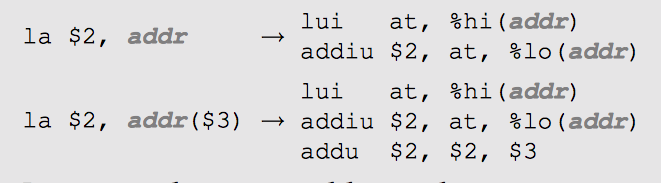
\includegraphics[width=1\textwidth]{hilo.png}
	\caption{Instruções equivalentes dos construtores \%hi() e \%lo(). Imagem retirada do livro \cite{mipsrun}.}
	\label{fig:hilo}
\end{figure}

Os construtores \%hi() e \%lo() também não estão presentes em todos montadores MIPS, podendo ser substituídos como mostra a Figura~\ref{fig:hilo}. Logo, as seguintes instruções foram trocadas :

\begin{itemize}
	\item lui \$v1,\%hi(\$LC0) e addiu \$a0,\$v1,\%lo(\$LC0) : la \$a0, \$LC0
    \item lui \$v0,\%hi(v) e addiu \$a0,\$v0,\%lo(v) : la \$a0, v
\end{itemize}

Outro problema encontrado foi na instrução \textit{j \$31, ou seja, j \$ra}. A instrução \textit{j} pula para um endereço alvo, e \$ra é um registrador, portanto esta instrução foi substituída por \textit{jr \$ra}.

Algumas subrotinas como \textit{printf e putchar} não são encontradas no assembly gerado mas são chamadas com a instrução \textit{jal}, portanto estas também foram retiradas.

Por fim, mesmo após estas modificações básicas de sintaxe para que o código possa ser executado no MARS, ainda assim o código possui o fluxo um pouco confuso, já que após o primeiro \textit{loop} ele já iria sair do processo com a instrução \textit{li \$a0, 10} que chama o serviço \textit{exit (terminate execution)}. Portanto, algumas modificações foram realizadas para que o fluxo deste programa se inicie no \textit{main}, chame as subrotinas \textit{show} e \textit{sort} e encerre no final da subrotina \textit{main}.

\subsubsection{Otimização do código Assembly}
\label{subsubsec:ot}

O arquivo \textit{sortc.c} foi compilado novamente usando 5 diretivas de compilação, \textit{-O0, -O1, -O2, -O3 e -Os}. Todos os arquivos gerados, \textit{sortc0.s}, \textit{sortc1.s}, \textit{sortc2.s}, \textit{sortc3.s} e \textit{sortcs.s} foram alterados de acordo com a subseção anterior para que fosse possível executá-los no \textit{MARS}. Também foram removidos os códigos para mostrar os números da ordenação na tela de \textit{debug} do \textit{MARS}.

Com ajuda do \textit{Mars} foram coletadas informações sobre o número de instruções executadas e a quantidade de memória utilizada nas otimizações \textit{sortc0.s} e \textit{sortc1.s} como é possível ver na Tabela~\ref{tab:opt}. A contagem das instruções e informações sobre a memória foram conferidas no menu \textit{Tools $>$ Instruction Statistics}.

\begin{table}[H]
	\centering
	\begin{tabular}{|c|c|c|}
		\hline
		\textbf{Arquivo} & \textbf{Instruções} & \textbf{Tamanho (Bytes)} \\\hline
		\textit{sortc.s} & 1748 & 890 \\\hline
		\textit{sortc0.s} & 1748 & 890 \\\hline
		\textit{sortc1.s} & 172 & 57 \\\hline
	\end{tabular}
	\caption{Códigos otimizados do arquivo \textit{sortc.c} utilizando o \textit{cross compiler mips-elf-gcc}.}
	\label{tab:opt}
\end{table}

Como podemos ver na Tabela~\ref{tab:opt} a otimização \textit{-O0} do arquivo citado do item \textit{1.1} da descrição do Laboratório 1, \textit{sortc.s}, não altera em nada a quantidade de instruções e memória utilizada, porém a primeira otimização (\textit{-O1}) já altera a quantidade de instruções executadas em uma proporção de aproximadamente 9.84 da original.

Não foi possível analisar as informações das otimizações \textit{-O2, -O3 e -Os} pois estes códigos emitiram erros de lógica e de instruções como é mostrado a seguir:

\begin{itemize}
	\item Os arquivos \textit{sortc2.s} e \textit{sortc3.s} emitiram o seguinte erro de lógica : \textit{line 105: Runtime exception at 0x0040010c: fetch address not aligned on word boundary 0xfffffffd}.
	\item O arquivo \textit{sortcs.s} continha um pseudo código \textit{bltzl $8,$L10} que o conjunto de instruções do \textit{Mars} não possui, portanto não foi possível executá-lo.
\end{itemize}

\subsection{Exercício 3. \textit{Sprites}}
\label{subsec:sprites}

Na resolução do exercício, utilizamos as \textit{sprites} do \textit{Ryu} para conseguir realizar a atividade de colisão proposta. A colisão acontece quando duas \textit{hitbox} de personagens distintos encostam entre si. O vídeo mostrando a interação de colisão pode ser vista neste \href{https://www.youtube.com/watch?v=kbTLQQuw6RA}{link}.


\subsection{Exercício 4. Cálculo das raízes da equação de segundo grau}
\label{subsec:raizes}

\begin{figure}[H]
	\centering
	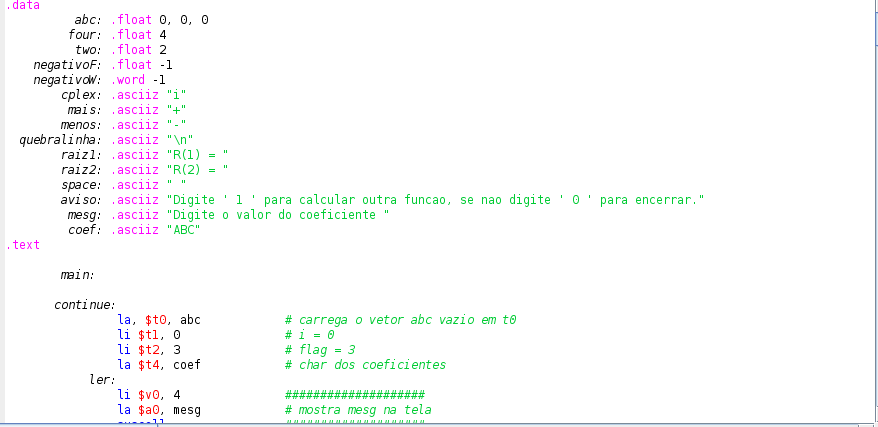
\includegraphics[width=1\textwidth]{EX_4_1.png}
	\caption{Código do exercício 4.}
	\label{fig:hilo1}
\end{figure}

\begin{figure}[H]
	\centering
	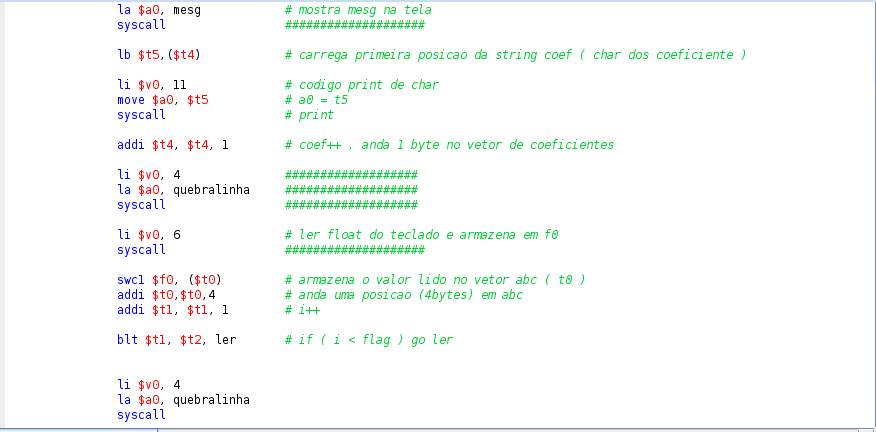
\includegraphics[width=1\textwidth]{EX_4_2.png}
	\caption{Código do exercício 4.}
	\label{fig:hilo2}
\end{figure}

\begin{figure}[H]
	\centering
	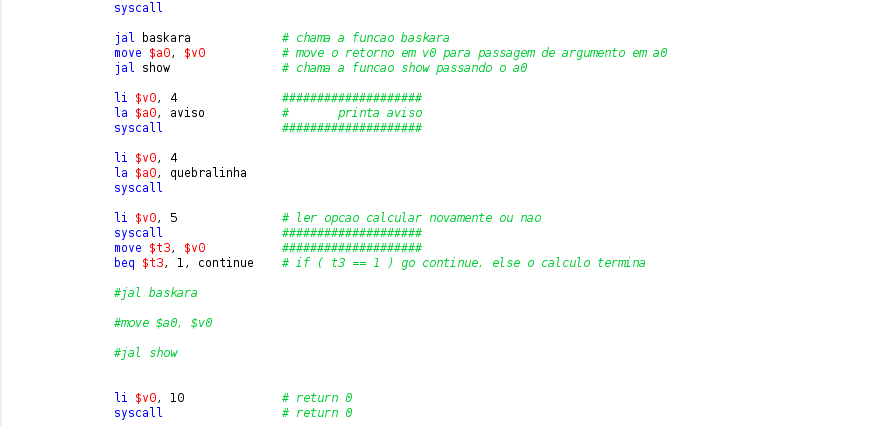
\includegraphics[width=1\textwidth]{EX_4_3.png}
	\caption{Código do exercício 4.}
	\label{fig:hilo3}
\end{figure}

\begin{figure}[H]
	\centering
	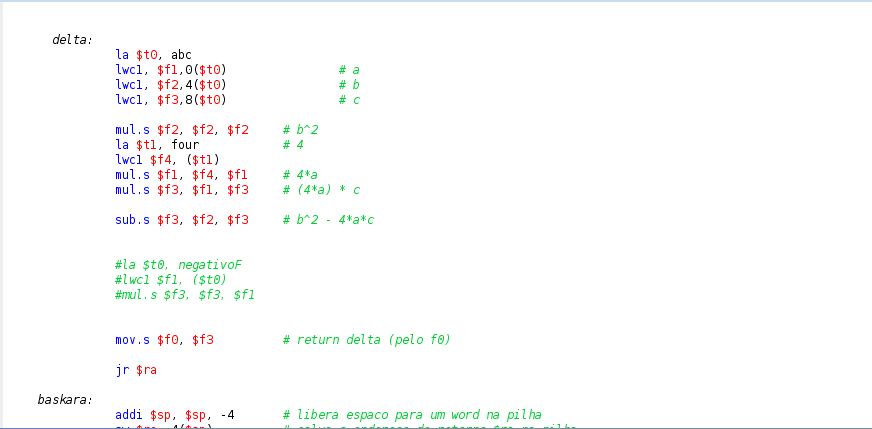
\includegraphics[width=1\textwidth]{EX_4_4.png}
	\caption{Código do exercício 4.}
	\label{fig:hilo4}
\end{figure}

\begin{figure}[H]
	\centering
	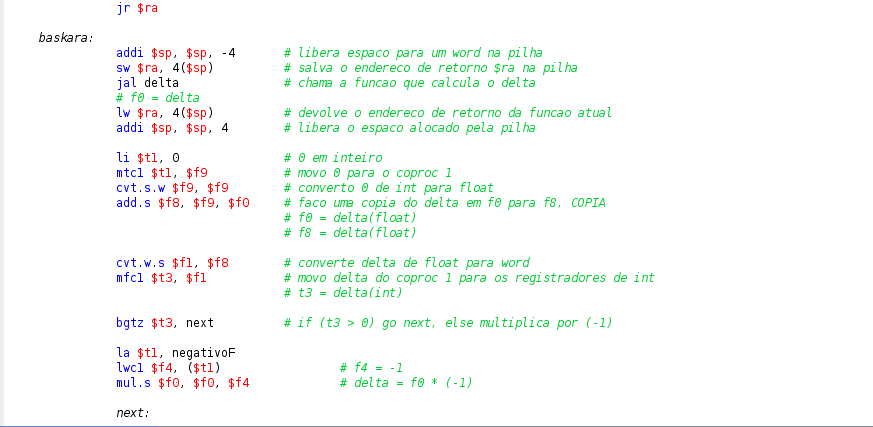
\includegraphics[width=1\textwidth]{EX_4_5.png}
	\caption{Código do exercício 4.}
	\label{fig:hilo5}
\end{figure}

\begin{figure}[H]
	\centering
	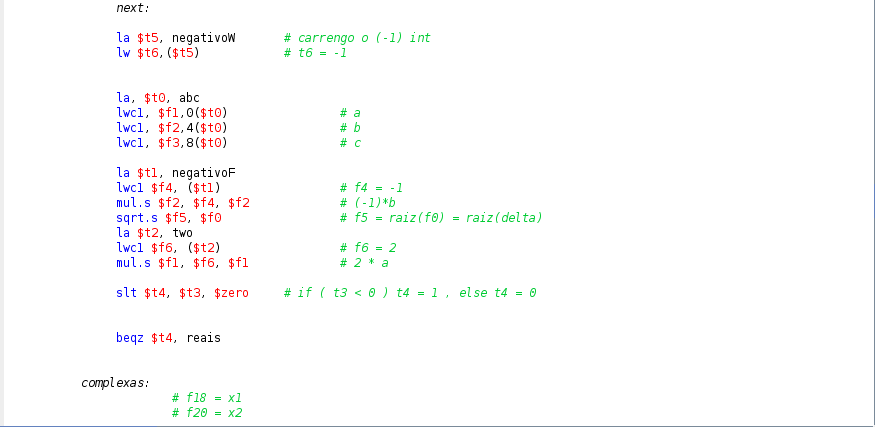
\includegraphics[width=1\textwidth]{EX_4_6.png}
	\caption{Código do exercício 4.}
	\label{fig:hilo6}
\end{figure}

\begin{figure}[H]
	\centering
	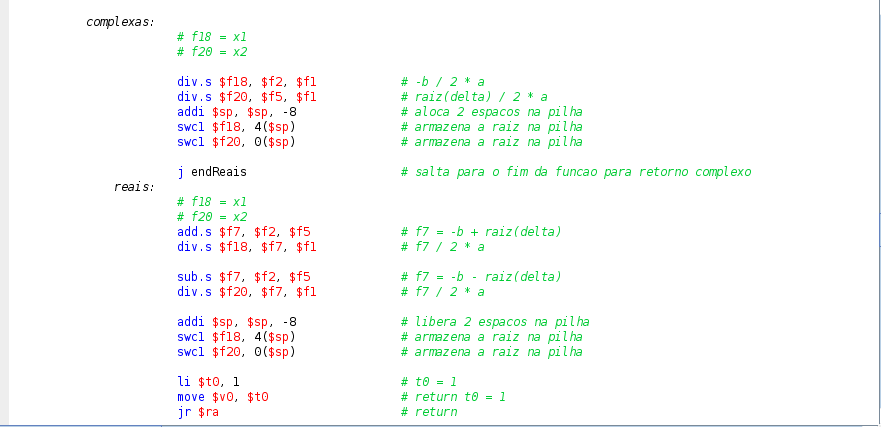
\includegraphics[width=1\textwidth]{EX_4_7.png}
	\caption{Código do exercício 4.}
	\label{fig:hilo7}
\end{figure}

\begin{figure}[H]
	\centering
	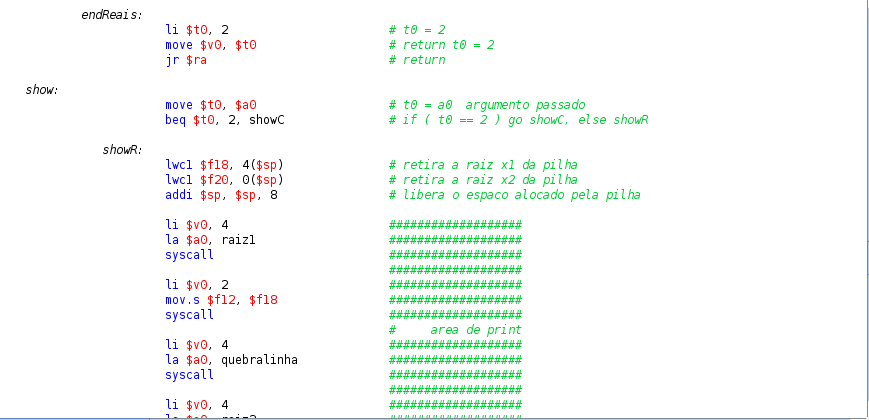
\includegraphics[width=1\textwidth]{EX_4_8.png}
	\caption{Código do exercício 4.}
	\label{fig:hilo8}
\end{figure}

\begin{figure}[H]
	\centering
	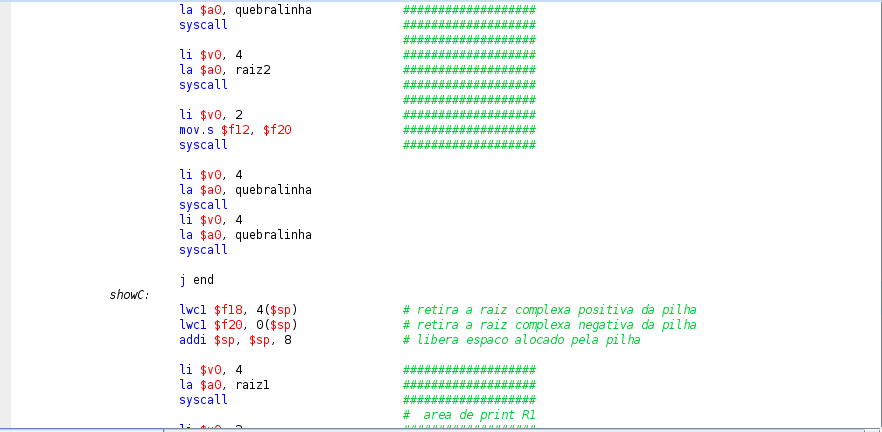
\includegraphics[width=1\textwidth]{EX_4_9.png}
	\caption{Código do exercício 4.}
	\label{fig:hilo9}
\end{figure}

\begin{figure}[H]
	\centering
	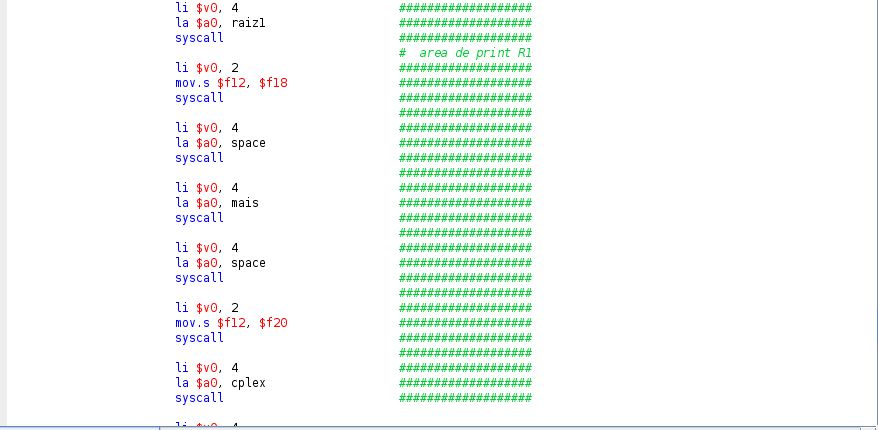
\includegraphics[width=1\textwidth]{EX_4_10.png}
	\caption{Código do exercício 4.}
	\label{fig:hilo10}
\end{figure}

\begin{figure}[H]
	\centering
	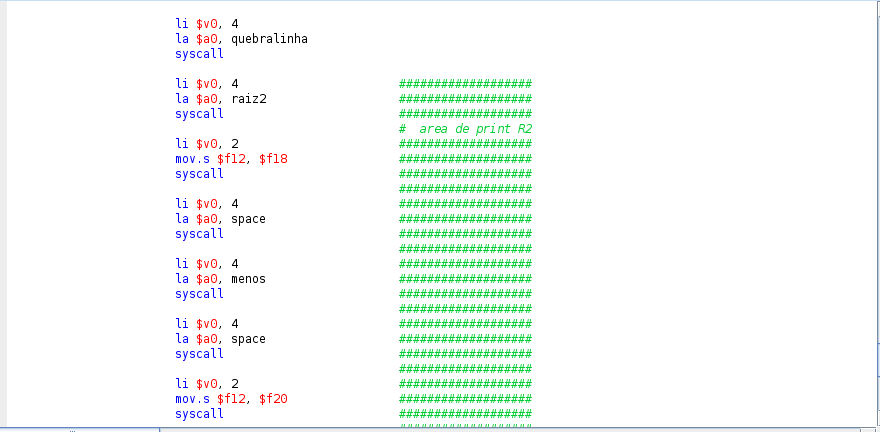
\includegraphics[width=1\textwidth]{EX_4_11.png}
	\caption{Código do exercício 4.}
	\label{fig:hilo11}
\end{figure}

\begin{figure}[H]
	\centering
	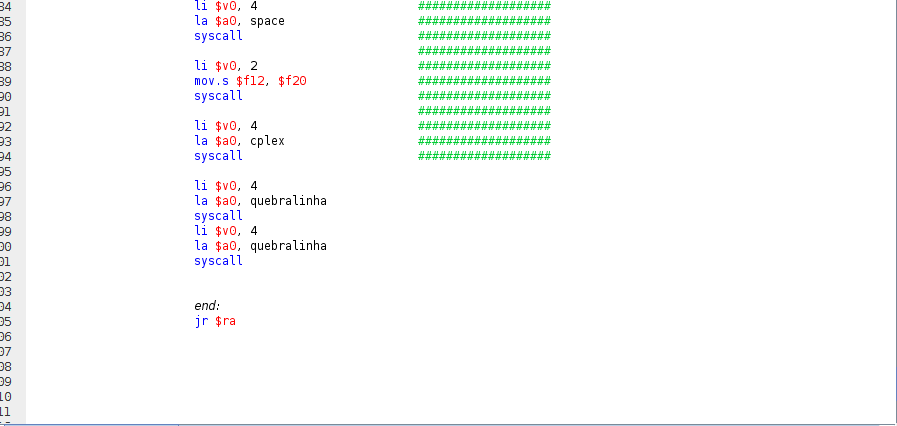
\includegraphics[width=1\textwidth]{EX_4_12.png}
	\caption{Código do exercício 4.}
	\label{fig:hilo12}
\end{figure}

\subsubsection{Teste de raízes reais e complexas}
\label{subsubsec:testebhas}

Criamos o procedimento \textit{baskara} especificado na Figura~\ref{fig:hilo5}, e chamamos a sub rotina \textit{delta}, cujo o código está comentado na Figura~\ref{fig:hilo4}. O programa retorna como resultado, 1 caso o valor de \textit{delta} for positivo (resultados reais), ou 2 caso for negativo (resultados imaginários).

\subsubsection{Show}
\label{subsubsec:show}

Utilizamos a função \textit{show} apresentada na Figura~\ref{fig:hilo8}, que por sua vez caso a mesma receber os valores 2 ou 1, chama \textit{showC} (função pra mostrar as raízes complexas), ou deixa prosseguir para \textit{showR} (cujo o procedimento é mostrar as raízes reais) respectivamente. Todas as sub rotinas para mostrar valores são apresentadas e comentadas na Figura~\ref{fig:hilo9},  Figura~\ref{fig:hilo10}, Figura~\ref{fig:hilo11} e Figura~\ref{fig:hilo12}.

\subsubsection{Main}
\label{subsubsec:Main}

Ao iniciar o programa é mostrado uma mensagem pedindo os coeficientes que utilizaremos na equação de segundo grau (usando os comandos de \textit{syscall} e os respectivos registradores para coletar as entradas do teclado). Ao receber os valores de entrada, é chamado a instrução \textit{baskara}, que por sua vez chama \textit{delta} e assim em sequência chama a sub rotina \textit{show}. No final da execução é mostrado os resultados e perguntamos ao usuário se ele deseja continuar utilizando o programa. Caso o usuário concordar em dar continuidade ao programa, a sub rotina \textit{continue} é chamada, que retorna ao começo do arquivo. Todos os processos são mostrados em todas figuras a partir da Figura~\ref{fig:hilo1}.

\subsubsection{Tempos de execução da rotina \textit{baskara}}
\label{subsubsec:4.4}

Nesta parte foi preciso calcular o \textit{texec} para vários valores, como nosso código não possui nenhum \textit{loop}, as instruções \textit{FR} e \textit{FI} são utilizadas em um número constante de vezes. Em outros tipos podem sofrer pequenas diferenças na quantidade de instruções. Foi fornecido que o código iria ser executado em um processador \textit{MIPS} de \textit{1GHZ}. Utilizamos a equação \(texec= C * T\) e chegamos aos seguintes resultados:

\begin{enumerate}
\item \([1, 0, -9.86960440]\)

	\(texec = 211 ns\)
\item \([1, 0, 0]\)

	\(texec = 222 ns\)
\item \([1, 99, 2459]\)

	\(texec = 219 ns\)

\item \([1, -2468, 33762440]\)

	\(texec = 219 ns\)
\item \([0, 10, 100]\)

	\(texec = 211 ns\)
\end{enumerate}

\subsection{Exercício 5. Trajetórias}

A simulação pedida no exercício 5 foi concluída parcialmente devido alguns problemas na representação dos \textit{pixels} na tela, os cálculos da física estão corretos, porém ao serem convertidos em \textit{pixels} e mostrados na tela não demonstravam o resultado esperado. O código escrito pode ser encontrado neste \href{https://github.com/Dayof/OAC172/blob/master/Lab1/ex5/lancamento.asm}{link}.

A demonstração foi concluída apenas na metade do trajeto, ou seja, a bola de canhão apenas subiu, assim não concluindo seu trajeto de queda como podemos ver na Figura~\ref{fig:traj}. Os valores testados nos cálculos foram de $v_{0x} = 14$ m/s e $v_{0y} = 10$ m/s.

\begin{figure}[H]
	\centering
	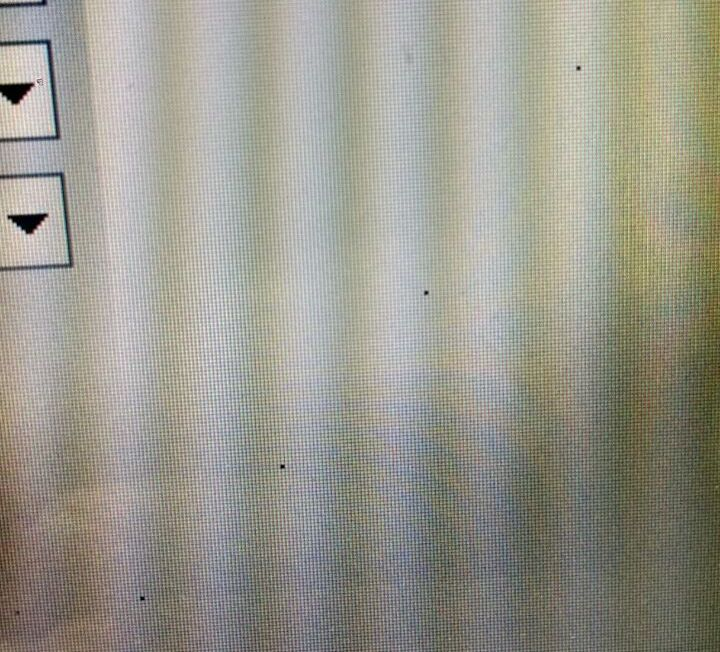
\includegraphics[width=.6\textwidth]{5.jpg}
	\caption{Trajetória de subida da bola do canhão.}
	\label{fig:traj}
\end{figure}

\bibliographystyle{sbc}
\bibliography{relatorio}

\end{document}
